\documentclass[twoside]{article}
\usepackage[a4paper]{geometry}
\geometry{verbose,tmargin=2.5cm,bmargin=2cm,lmargin=2cm,rmargin=2cm}
\usepackage{fancyhdr}
\pagestyle{fancy}

% nastavení pisma a češtiny
\usepackage{lmodern}
\usepackage[T1]{fontenc}
\usepackage[utf8]{inputenc}
\usepackage[czech]{babel}

% odkazy
\usepackage{url}

% vícesloupcové tabulky
\usepackage{multirow}
\usepackage{amssymb}
\usepackage{bbold}
\usepackage{amsmath}
\usepackage{commath}

% vnořené popisky obrázků
\usepackage{subcaption}

% automatická konverze EPS 
\usepackage{graphicx} 
\usepackage{epstopdf}
\epstopdfsetup{update}

\graphicspath{{./images}}

% odkazy a záložky
\usepackage[unicode=true, bookmarks=true,bookmarksnumbered=true,
bookmarksopen=false, breaklinks=false,pdfborder={0 0 0},
pdfpagemode=UseNone,backref=false,colorlinks=true] {hyperref}

% Poznámky při překladu
\usepackage{xkeyval}	% Inline todonotes
\usepackage[textsize = footnotesize]{todonotes}
\presetkeys{todonotes}{inline}{}

% Zacni sekci slovem ukol
\renewcommand{\thesection}{Úkol \arabic{section}}
% enumerate zacina s pismenem
\renewcommand{\theenumi}{\alph{enumi}}

% smaz aktualni page layout
\fancyhf{}
% zahlavi
\usepackage{titling}
\fancyhf[HC]{\thetitle}
\fancyhf[HLE,HRO]{\theauthor}
\fancyhf[HRE,HLO]{\today}
 %zapati
\fancyhf[FLE,FRO]{\thepage}

% údaje o autorovi
\title{Automatické řízení: DÚ 1 - Linearizace}

\author{Vojtěch Michal}
\date{\today}

\begin{document}

\maketitle

\textbf{Zadání:}

Uvažujte model podélné dynamiky vozu pohybujícího se rychlostí v po vozovce se sklonem $\alpha$. Systém
lze popsat následujícími diferenciálními rovnicemi:
\begin{equation}
	\begin{split}
		m\dot{v} = c_\lambda \cdot \left(\frac{\omega \cdot r}{v} - 1 \right) - m \cdot g \cdot \text{sin} \alpha - k_{Drag} \cdot v^2 \\
		J \dot{\omega} = -m \cdot \dot{v} \cdot r + T_q,
	\end{split}
	\label{eq:zadani}
\end{equation}
kde $v(t)$ [m/s] je podélná
rychlost vozu v těžišti, $\omega(t)$ [1/s]
je úhlová rychlost hnaných
kol, $T_q(t)$ [Nm] je trakční
moment vozu. Zbylé koeficienty
jsou uvedené v tabulce, kde $m$ je
hmotnost vozu, $r$ je poloměr kol,
$c_\lambda $ je konstanta určující trakční
sílu hnaného kola, $k_{Drag} [Ns^2m^-2]$ je konstanta aerodynamického odporu vozu, $\alpha (t)$ [rad] je sklon
vozovky, a $J$ je moment setrvačnosti kola. Vstup systému $T_q(t)$ je omezen na interval <0, 10 000 Nm >.
 V autě je umístěn senzor, kterým lze měřit pouze podélnou rychlost vozu, což je jediným výstupem systému.

 \begin{table}[htbp]
	 \centering
	 \begin{tabular}{c|c|c|c|c|c|c|c}
		Proměnná & $m$ & $r$ & $k_{Drag}$ & $\alpha(t)$ & $g$ & $c_\lambda$ & $J$ \\
		\hline
		Hodnota & 1000 & 0.33 & 0.4513 & <-0.1, 0.1> & 9.81 & 50 000 & 22500 \\
		\hline
		Jednotky & kg & m & $Ns^2m^{-2} $ & rad & $m/s^2 $ & N/rad & $kg m^2$		 
	 \end{tabular}
 \end{table}
Systém má dva vnitřní stavy $v$ a $\omega$, které dohromady tvoří vektor ve stavovém prostoru. Označím jej $\vec{x}$.
\begin{equation}
	\vec{x}(t) = \begin{bmatrix}
		x_1(t) = v(t) \\
		x_2(t) = \omega(t)
	\end{bmatrix}
\end{equation}

% ---------------------------------
% ---------------------------------
% název sekce je generován automaticky jako: Úkol X
\section{}
\label{sec:ukol1}
Implementujte nelineární model v Simulinku. Nezapomeňte na statické nelinearity tohoto systému.
Provedeno, nepotřebuje komentář.

\section{}
\label{sec:ukol2}
Proveďte lineární aproximaci modelu v pracovním bodě $P$ s hodnotami $\alpha(t) = \frac{\pi}{36}$ rad, $v(0) = 15$ m/s.

\subsection{}
Analytická podmínka pro rovnovážný pracovní bod P: v rovnovážném pracovním bodě je derivace vnitřních stavů nulová, tedy $\dot{\vec{x}}_P = 0$.
Dosazením do \eqref{eq:zadani} získáme pro vstup v pracovním bodě
\begin{equation}
	0 = 0 + T_q
\end{equation}
a pro $\omega$
\begin{equation}
	\begin{split}
		0 = c_\lambda \cdot \left(\frac{\omega_p \cdot r}{v_p} - 1 \right) - m \cdot g \cdot \text{sin} \alpha - k_{Drag} \cdot v_p^2, \\
		m \cdot g \cdot \text{sin} \alpha + k_{Drag} \cdot v_p^2 =  c_\lambda \cdot \left(\frac{\omega_p \cdot r}{v_p} - 1 \right) \\
		\frac{1}{c_\lambda}(m \cdot g \cdot \text{sin} \alpha + k_{Drag} \cdot v_p^2) + 1 =  \frac{\omega_p \cdot r}{v_p} \\
		\omega_p = \frac{v_p}{r} \cdot(\frac{1}{c_\lambda}(m \cdot g \cdot \text{sin} \alpha + k_{Drag} \cdot v_p^2) + 1)\\
		\omega_p = \frac{15}{0.33} \cdot\left(\frac{1}{50000}\left(1000 \cdot 9.81 \cdot \text{sin}(\frac{\pi}{36}) + 0.4513 \cdot 15^2\right) + 1\right) = 46.3241
	\end{split}
\end{equation}
Tím jsme nalezli pracovní bod $P = \begin{bmatrix}
	v_p & \omega_p & T_{qp}
\end{bmatrix} = \begin{bmatrix}
	15 \text{m/s} & 46.3241 \text{rad/s} & 0 \text{Nm}
\end{bmatrix} $.

\subsection{}
Linearizujme v pracovním bodě $P$. Hledám matice A, B, C, D lineárního systému, které budou aproximovat původní nelineání popis \eqref{eq:zadani} na okolí bodu $P$.
Potřebuji linearizovat nelineární vektorovou funkci $f(\vec{x}, T_q) = (f_1, f_2)$ danou po složkách předpisy
\begin{equation}
		\dot{v} = f_1(\vec{x}, T_q) = \frac{c_\lambda \cdot \left(\frac{\omega \cdot r}{v} - 1 \right) - m \cdot g \cdot \text{sin} \alpha - k_{Drag} \cdot v^2}{m}
		= c_\lambda \frac{\omega \cdot r}{mv} - \frac{c_\lambda}{m} - g \cdot \text{sin} \alpha - \frac{k_{Drag}}{m} \cdot v^2
	\end{equation}
	\begin{equation}
		\begin{split}
			\dot{\omega} = f_2(\vec{x}, T_q) = \frac{-(c_\lambda \cdot \left(\frac{\omega \cdot r}{v} - 1 \right) - m \cdot g \cdot \text{sin} \alpha - k_{Drag} \cdot v^2) \cdot r + T_q}{J} = \\
			= -c_\lambda \frac{\omega \cdot r^2}{Jv} + \frac{c_\lambda r}{J}  + \frac{r \cdot m \cdot g}{J} \cdot \text{sin} \alpha + \frac{k_{Drag}}{J} \cdot v^2 + \frac{T_q}{J}
		\end{split}
	\end{equation}
Z těchto funkcí pomocí parciálních derivací nalezneme prvky hledaných matic. Matice C plyne rovnou ze zadání. Matice B, D lze určit snadno pohledem na rovnice:
\begin{equation}
	D = 0 ~~~~~~~~ C = \begin{bmatrix}
		1 & 0
	\end{bmatrix} ~~~~~~~ B = \begin{bmatrix}
		0 \\ J^{-1}
	\end{bmatrix} = \begin{bmatrix}
		0 \\ \frac{1}{2250}
	\end{bmatrix}.
\end{equation}
Matice A bude složitější na výpočet, parciální derivace musíme vyčíslit v pracovním bodě: 
\begin{equation}
	A = \begin{bmatrix}
		\frac{\partial f_1}{\partial v} & \frac{\partial f_1}{\partial \omega} \\ 
		\frac{\partial f_2}{\partial v} & \frac{\partial f_2}{\partial \omega}
	\end{bmatrix}_P = \begin{bmatrix}
		-c_\lambda \frac{w_p \cdot r}{m v_p^2} - \frac{k_{Drag}}{m}2v_p & c_\lambda \frac{r}{m v_p} \\
		c_\lambda \frac{w_p \cdot r^2}{J v_p^2} + \frac{k_{Drag}}{J}2v_p & -c_\lambda \frac{r^2}{J v_p}
	\end{bmatrix}.
\end{equation}
Po dosazení
\begin{equation}
	A = \begin{bmatrix}
		-50000 \frac{46.3241 \cdot 0.33}{1000 \cdot 225} - 30 \cdot \frac{0.4513}{1000} & 50000 \frac{0.33}{1000 \cdot 15} \\
		50000 \frac{46.3241 \cdot 0.33^2}{2250 \cdot 225} + 30 \cdot \frac{0.4513}{2250} & -50000 \frac{0.33^2}{2250 \cdot 15} \\
	\end{bmatrix} = \begin{bmatrix}
		-3.4106 & 1.1 \\
		0.5043 & 0.1613 \\
	\end{bmatrix}.
\end{equation}
S pomocí těchto matic lze zapsat lineární aproximaci systému v odchylkovém tvaru jako
\begin{equation}
	\begin{split}
		\Delta \dot{\vec{x}} &= A \Delta \vec{x} + B \Delta u, \\
		\Delta y &= C \Delta\vec{x} + D \Delta u, \\
	\end{split}
\end{equation}
kde přeznačím $u = T_q$, abych se držel standardu v teorii řízení.
	
\begin{figure}[htbp]
    \centering % <-- added
\begin{subfigure}{0.45\textwidth}
  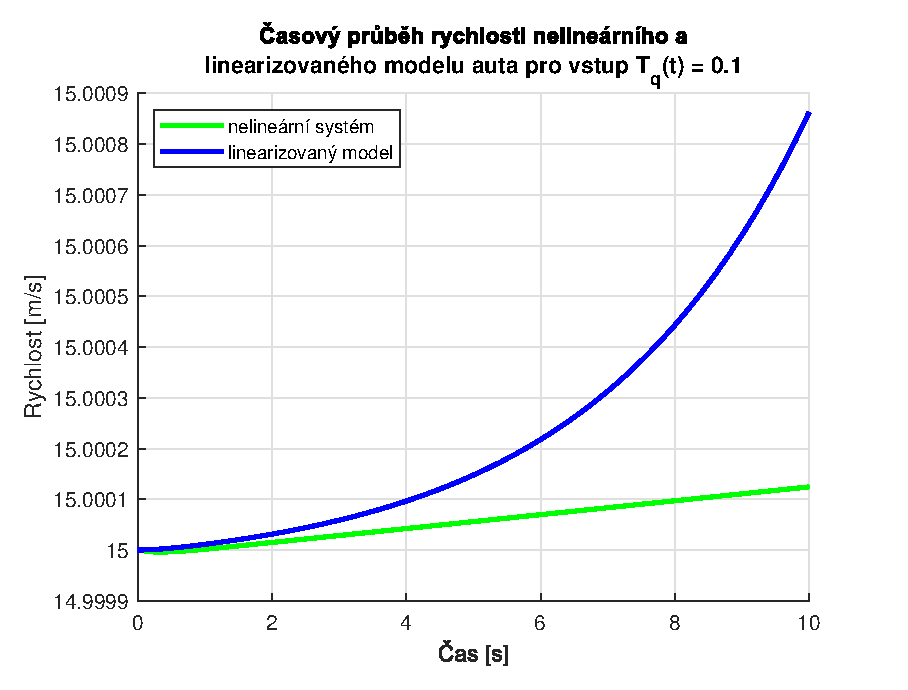
\includegraphics[width=\linewidth]{uloha12-01.eps}
  \caption{Simulace pro vstup $T_q(t) = 0.1$}
\end{subfigure}\hfil % <-- added
\begin{subfigure}{0.45\textwidth}
	\includegraphics[width=\linewidth]{uloha12-100.eps}
	\caption{Simulace pro vstup $T_q(t) = 100$}
\end{subfigure}
\caption{Srovnání odezvy nelineárního a linearizovaného modelu na step function}
\label{fig:nelin-100}
\end{figure}

\subsection{}
Odezva nelineárního systému a linearizovaného modelu je k porovnání na obrázcích \ref{fig:nelin-100}. Simulace proběhla
pro konstantní vstupy $T_{q1} = 0.1$ a $T_{q2} = 100$. Vzhledem k tomu. že linearizace proběhla v pracovním bodě s $T_p = 0$,
je očekávatelné, že výstup pro $T_{q1}$ bude blíže referenčnímu výstupu z nelineárního modelu. Lineární aproximace však
má tendenci růst mnohem rychleji jak odezva nelineárního systému.
Pro validaci linearizace by se tak hodil vstupní signál střídavě rostoucí a klesající. Na obrázku \ref{fig:nelin-sin}
jsou vykresleny průběhy pro harmonický a obdélního vý vstupní signál. Lineární model vykazuje stejný charakter
zvlnění jako model nelineární, nad to je ale stále v jeho odezvě superponována rostoucí exponenciála.
\begin{figure}[htbp]
    \centering % <-- added
\begin{subfigure}{0.45\textwidth}
  \includegraphics[width=\linewidth]{uloha12-sin.eps}
  \caption{Simulace pro sinusový vstup }
\end{subfigure}\hfil % <-- added
\begin{subfigure}{0.45\textwidth}
	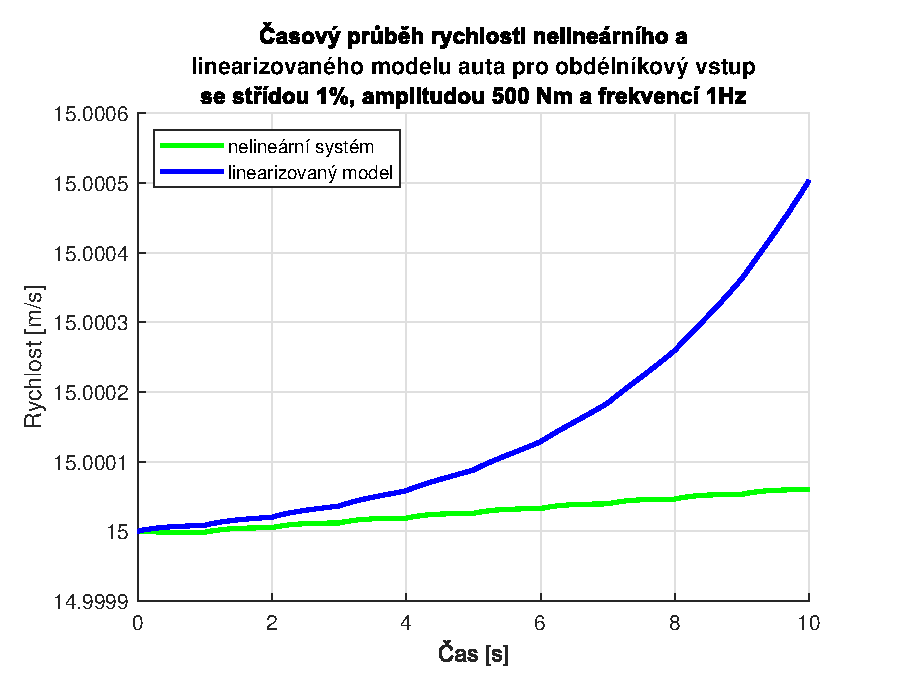
\includegraphics[width=\linewidth]{uloha12-square.eps}
	\caption{Simulace pro obdélníkový vstup }
\end{subfigure}
\caption{Srovnání odezvy nelineárního a linearizovaného modelu na periodické funkce}
\label{fig:nelin-sin}
\end{figure}


\section{}
\label{sec:ukol3}
Proveďte lineární aproximaci modelu v případě rovnoměrné akcelerace vozu $\dot{v}(t) = 1 [ m/s^2]$ a jízdě
po rovině ($\alpha(t) = 0$°, $v(0) = 0.5$ m/s).

Díky podmínce $\alpha = 0$ se rovnice \eqref{eq:zadani} zjednoduší na
\begin{equation}
	\begin{split}
		m\dot{v} = c_\lambda \cdot \left(\frac{\omega \cdot r}{v} - 1 \right) - k_{Drag} \cdot v^2, \\
		J \dot{\omega} = -m \cdot \dot{v} \cdot r + T_q.
	\end{split}
	\label{eq:rovina}
\end{equation}
Dále je z podmínky $\dot{v} = 1$ a počáteční podmínky $v(0) = 0.5$ vidět předpis $v(t) = t + 0.5$
Zvolená pracovní trajektorie je popsaná funkcemi $\vec{x_p}(t)$ a $T_{qp}(t)$, výstup je stále přímo stavová proměnná $x_1(t)$.
Dosazením průběhu $\dot{v_p}(t)$ do \eqref{eq:rovina} hledáme předpis pro $\omega_p(t)$ a $T_{qp}(t)$, obecně již neplatí výhodná vlastnost ekvilibria, že by derivace byly nulové.
Z první rovnice získáme časový průběh $\omega_p(t)$ na pracovní trajektorii, z rovnice druhé pro $T_{qp}(t)$.
\begin{equation}
	\begin{split}
		m &= c_\lambda \cdot \left(\frac{\omega_p(t) \cdot r}{v_p(t)} - 1 \right) - (v_p(t))^2 \cdot k_{Drag} \\
		\frac{m + (v_p(t))^2 \cdot k_{Drag}}{c_\lambda} &= \frac{\omega_p(t) \cdot r}{v_p(t)} - 1 \\
		\omega_p(t) &= \frac{v_p(t)}{r} \left(\frac{m + (v_p(t))^2 \cdot k_{Drag}}{c_\lambda} + 1\right). \\
	\end{split}
	\label{eq:omegap}
	\end{equation}
Po numerickém dosazení:
\begin{equation}
	\begin{split}
	\omega_p(t) = \frac{0.5 + t}{0.33} (\frac{1000 + (t^2 + t + \frac{1}{4}) \cdot 0.4513}{50000} + 1)
	= \frac{100t + 50}{33} \cdot \frac{1000 + 0.4513 \cdot (t^2 + t + \frac{1}{4}) + 50000}{50000} = \\
	= (2t + 1) \cdot \frac{0.4513 \cdot (t^2 + t + \frac{1}{4}) + 51000}{33000} = \frac{51}{33} (2t+1) + \underbrace{\frac{0.4513}{33000} (2t^3 + 3t^2 + 1.5t + 0.25)}_{\text{skoro nula kvůli koeficientu ~} 10^{-5} } = \frac{51}{33}(2t+1)
	\end{split}
\end{equation}
Získaný předpis pro úhlovou rychlost kol zjednoduším na $\omega_p(t) =  \frac{51}{33}(2t+1)$ zanedbáním členů s malým skalárním koeficientem.
Dosaďme do druhé rovnice pro $T_{qp}(t)$:
	\begin{equation}
		\begin{split}
			J \underbrace{\dot{\omega}}_{=\frac{102}{33}} &= -m \cdot r + T_q(t) \\
			T_q(t) &= m \cdot r + \frac{102}{33} J = 7284 \text{Nm}
		\end{split}
	\end{equation}
A tím jsme nalezli pracovní bod $P$.

\subsection{}
\subsection{}
% ---------------------------------
% ---------------------------------
% Literatura
\begin{thebibliography}{9}

% vzorová citace
\bibitem{lamport94}
  Leslie Lamport,
  \emph{\LaTeX: A Document Preparation System}.
  Addison Wesley, Massachusetts,
  2nd Edition,
  1994.

\bibitem{Wiki}
	\LaTeX tutorials, \url{http://en.wikibooks.org/wiki/LaTeX/}

\bibitem{motivace}
	Motivační hudba, \emph{Kirby dream land theme song} \url{https://www.youtube.com/watch?v=3CS93CdMv_E}

\bibitem{ARI11}
	Studenti předmětu ARI 2011, \emph{ARI song (videoklip)} \url{http://www.youtube.com/watch?v=5gDfQK7dD7c}
\end{thebibliography}












\end{document}

